\documentclass[a4paper,11pt,fleqn]{scrartcl}%fleqn pour aligner les equations à gauche
\usepackage{../../Styles/Cours}


\newcommand{\chnum}{Chapitre 14}
\newcommand{\chtitle}{Modélisation de l'écoulement d'un fluide}
\newcommand{\dtype}{Cours}
  
\begin{document}
	\maketitle

\section{Modèle du fluide incompressible}
    \subsection{Définition et validité}
    L'état "fluide" est définit comme étant un milieu matériel déformable, ce qui comprend en particulier la matière à l'état liquide ou gazeux. Un fluide incompressible est caractérisé par le fait que sa masse volumique soit constante : $\rho = cste$\\
    Ce modèle est applicable à un fluide quand la température est constante, homogène et si la vitesse d'écoulement $v$ est petite devant la célérité $c$ des ondes acoustiques qui pourraient s'y propager.
    
    \subsection{La poussée d'Archimède}
    La résultante  des forces pressantes exercées sur un corps plongé dans un fluide incompressible au repos de masse volumique $\rho$ est appelée \textbf{poussée d'Archimède} et notée $\overrightarrow{\pi_A}$. Elle est égale à l'opposé du poids du fluide déplacée lors de l'immersion.\\
    Pour un corps ayant un volume immergé $V$, l'expression vectorielle de la poussée d'Archimède est :
    \begin{center}
        \begin{tabular}{c|c}
        \multirow{3}{*}{$\overrightarrow{\pi_A}=-\rho V \overrightarrow{g}$} & avec $\rho$ en \unit{\kilo\gram\per\meter\cubed}\\
        &$V$ en \unit{\meter\cubed}\\
        &$g = \SI{9.81}{\newton\per\kilo\gram}$\\
    \end{tabular}
    \end{center}
    La poussée d'Archimède est une conséquence de l'augmentation de la pression (et de la force pressante) avec la profondeur dans un fluide incompressible.
    
    \begin{figure}[h!]
    \caption*{\textbf{Forces pressantes exercées par un fluide sur un solide immergé}}
    \centering
    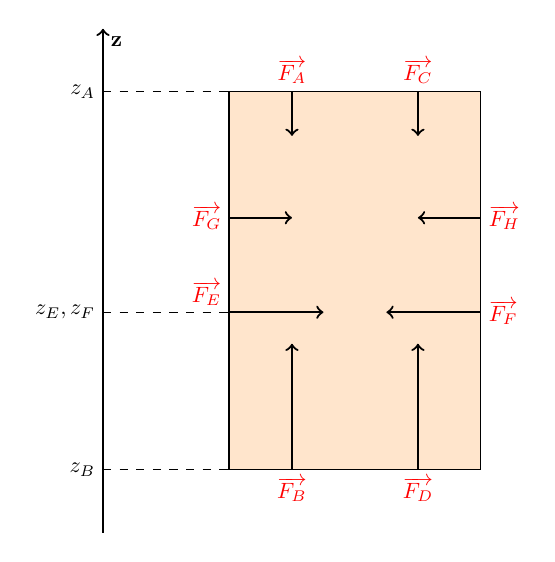
\begin{tikzpicture}[scale=.8,transform shape]
    	\fill[orange!20] (2,0) rectangle(6,6);
    	\draw (2,0) rectangle(6,6);
    	\draw[->, thick] (0,-1) to (0,7);
    	\draw[dashed] (0,6) --(2,6);
    	\draw[dashed] (0,2.5) --(2,2.5);
    	\draw[dashed] (0,0) --(2,0);
    	\draw[->,thick] (3,6) to (3,5.3);
    	\draw[->,thick] (5,6) to (5,5.3);
    	
    	\draw[->,thick] (2,4) to (3,4);
    	\draw[->,thick] (6,4) to (5,4);
    	
    	\draw[->,thick] (2,2.5) to (3.5,2.5);
    	\draw[->,thick] (6,2.5) to (4.5,2.5);
    	
    	
    	\draw[->,thick] (3,0) to (3,2);
    	\draw[->,thick] (5,0) to (5,2);
    	
    	\node[below right] (z) at (0,7){\textbf{z}};
    	\node[left] (zA) at (0,6){$z_A$};
    	\node[left] (zInt) at (0,2.5){$z_E,z_F$};
    	\node[left] (zB) at (0,0){$z_B$};
    	
    	\node[above, red] (FA) at (3,6){$\overrightarrow{F_A}$};
    	\node[above, red] (FC) at (5,6){$\overrightarrow{F_C}$};
    	\node[left, red] (FG) at (2,4){$\overrightarrow{F_G}$};
    	\node[left, red] (FE) at (2,2.8){$\overrightarrow{F_E}$};
    	\node[right, red] (FH) at (6,4){$\overrightarrow{F_H}$};
    	\node[right, red] (FF) at (6,2.5){$\overrightarrow{F_F}$};
    	\node[below, red] (FB) at (3,0){$\overrightarrow{F_B}$};
    	\node[below, red] (FD) at (5,0){$\overrightarrow{F_D}$};
    \end{tikzpicture}
    \end{figure}
\section{Écoulement d'un fluide}
    \subsection{Écoulement d'un fluide en régime permanent}
    Pour décrire l'écoulement d'un fluide incompressible, on subdivise le fluide en unités appelées "particules de fluide", une particule de fluide étant un système fermé de dimensions mésoscopiques.\\
    Les vecteurs vitesse des particules de fluides sont tangent en tout point à des courbes appelées lignes de champ de vitesse ou ligne de courant. Elles permettent de cartographier le champ de vitesse du fluide.\\
    L'écoulement est en \textbf{régime permanent} si la vitesse d'écoulement en tout point ne varie pas au cours du temps.\\
    \textbf{Dimensions mésoscopiques :} une particule de fluide a des dimensions mésoscopiques (typiquement \SI{0.1}{\micro\meter}), c'est-à-dire qu'elle est petite par rapport à l'échelle macroscopique mais suffisamment grande pour contenir un grand nombre d'entités microscopiques.

    \subsection{Conservation du débit volumique}
    Le \textbf{débit volumique} $D_V$ d'un fluide correspond au volume $V$ de fluide qui traverse une section droite par unité de temps :
    \begin{center}
        \begin{tabular}{c|m{7cm}}
        \multirow{3}{*}{$D_V=\dfrac{V}{\Delta t}$} & avec $D_V$ en \unit{\meter\cubed\per\second}\\
        &$V$ en \unit{\meter\cubed}\\
        &$\Delta t$, la durée en \unit{\second} pendant laquelle le volume $V$ traverse la section droite\\
    \end{tabular}
    \end{center}
    Le volume $V$ de fluide qui traverse une section droite d'aire $S$ pendant une durée $\Delta t$, avec une vitesse d'écoulement $v$, est contenu dans un cylindre de longueur $L=v\times \Delta t$ et de base d'aire $S$. Le débit volumique de fluide s'exprime :
    \begin{center}
        \begin{tabular}{c|c}
        \multirow{3}{*}{$D_V = \dfrac{v\cdot S\cdot \Delta t}{\Delta t} = v\cdot S$} & avec $D_V$ en \unit{\meter\cubed\per\second}\\
        &$v$ en \unit{\meter\per\second}\\
        &$S$ en \unit{\meter\squared}\\
    \end{tabular}
    \end{center}
    Pour un fluide incompréhensible, le débit volumique est le même en tout point d'un conduit. Si l'aire de la section droite du conduit change, la relation suivante, appelée équation de continuité, est vérifiée : $$D_{V1} = D_{V2} \leftrightarrow v_1 \cdot S_1 = v_2 \cdot S_2$$
\begin{multicols}{2}
	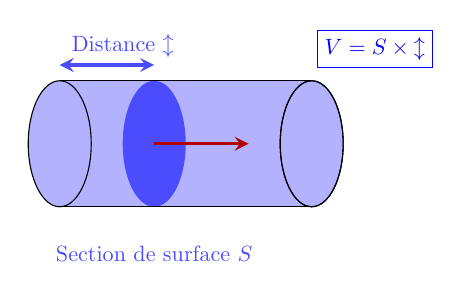
\begin{tikzpicture}[scale=.8,transform shape]
	\fill[blue!30] (0,0) rectangle(4,2);
	\fill[blue!70] (1.5,1) ellipse(.5 and 1);
	\fill[blue!30] (0,1) ellipse(.5 and 1);
	\fill[blue!30] (4,1) ellipse(.5 and 1);
	\draw (4,1) ellipse(.5 and 1);
	\draw (0,1) ellipse(.5 and 1);
	\draw (0,0)--(4,0);
	\draw (0,2)--(4,2);
	
	\draw[-stealth, red!70!black,very thick] (1.5,1) to (3,1);
	\node[draw, blue] (formula) at (5,2.5){$V=S\times \mathcal{l}$};
	\draw[stealth-stealth](4,1) ellipse(.5 and 1); (0,2.25) to (1.5,2.25);
	
	\draw[stealth-stealth,blue!70, very thick] (0,2.25) to (1.5,2.25);
	\node[below, blue!70] (S) at (1.5,-.5){Section de surface $S$};
	\node[above, blue!70] (l) at (1,2.25){Distance $\mathcal{l}$};
	\end{tikzpicture}

	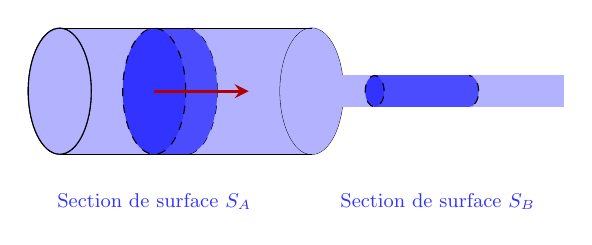
\begin{tikzpicture}[scale=.8,transform shape]
	\fill[blue!30] (0,0) rectangle(4,2);
	\draw[dashed] (2,1) ellipse(.5 and 1);
	\fill[blue!70] (1.5,0) rectangle(2,2);
	\fill[blue!70] (2,1) ellipse(.5 and 1);
	\fill[blue!80] (1.5,1) ellipse(.5 and 1);
	
	\draw (4,1) ellipse(.5 and 1);
	
	\draw[dashed] (1.5,1) ellipse(.5 and 1);
	
	
	\fill[blue!30] (0,1) ellipse(.5 and 1);
	\fill[blue!30] (4,1) ellipse(.5 and 1);
	\draw (0,1) ellipse(.5 and 1);
	
	
	\fill[blue!30] (4,.75) rectangle(8,1.25);
	
	\fill[blue!70] (6.5,1) ellipse(.15 and .25);
	\draw[dashed] (6.5,1) ellipse(.15 and .25);
	\fill[blue!70] (5,.75) rectangle(6.5,1.25);
	\fill[blue!80] (5,1) ellipse(.15 and .25);
	\draw[dashed] (5,1) ellipse(.15 and .25);
	
	\fill[blue!30] (0,1) ellipse(.5 and 1);
	\fill[blue!30] (4,1) ellipse(.5 and 1);
	\draw (0,1) ellipse(.5 and 1);
	\draw (0,0)--(4,0);
	\draw (0,2)--(4,2);
	
	\draw[-stealth, red!70!black,very thick] (1.5,1) to (3,1);
	%\node[draw, blue] (formula) at (5,2.5){$V=S\times \mathcal{l}$};
	%\draw[stealth-stealth,blue!70, very thick] (0,2.25) to (1.5,2.25);
	\node[below, blue!80] (S) at (1.5,-.5){\small Section de surface $S_A$};
	\node[below, blue!80] (S) at (6,-.5){\small Section de surface $S_B$};
	%\node[above, blue!70] (l) at (1,2.25){Distance $\mathcal{l}$};
	\end{tikzpicture}
\end{multicols}
	
    \subsection{Relation de Bernoulli et effet Venturi}
    Quand les frottement sont négligeables, l'écoulement d'un fluide incompressible de masse volumique $\rho$ constante, en régime permanent, vérifie la \textbf{relation de Bernoulli} entre deux points $M_1$ et $M_2$ :
    \begin{center}
        \begin{tabular}{m{7cm}|m{5cm}}
        \multirow{4}{*}{$P_1 + \rho g z_1 + \frac{1}{2}\rho v_1^2 = P_2 + \rho g z_2 + \frac{1}{2}\rho v_2^2$} & Pressions $P_1$ et $P_2$ en \unit{\pascal}\\
        &$\rho$ en \unit{\kilo\gram\per\meter\cubed}\\
        &Altitudes $z_1$ et $z_2$, en \unit{\meter}\\
        &$g = \SI{9.81}{\newton\per\kilo\gram}$\\
    \end{tabular}
    \end{center}
    Cette relation résulte d'un bilan d'énergie volumique. Elle s'applique pour des points sur une même ligne de courant, ou pour tous les points au sein du fluide si l'écoulement est non tourbillonnaire (irrotationnel).\\
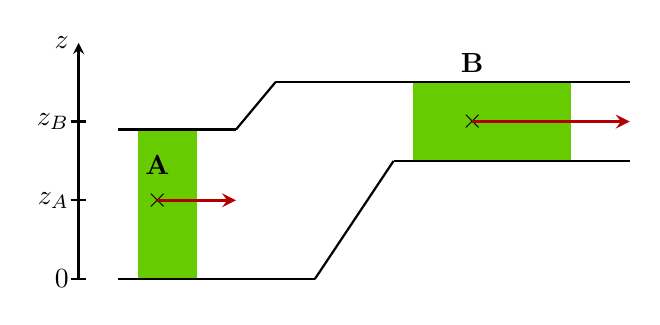
\begin{tikzpicture}
	\fill[green!60!orange] (.75,0) rectangle(1.5,1.9);
	\fill[green!60!orange] (4.25,1.5) rectangle(6.25,2.5);
	
	\draw[-stealth,thick] (0,0) to (0,3);
	\draw[thick] (-.1,0) -- (.1,0);
	\draw[thick] (-.1,1) -- (.1,1);
	\draw[thick] (-.1,2) -- (.1,2);
	\node[left] (0) at (0,0){$0$};
	\node[left] (zA) at (0,1){$z_A$};
	\node[left] (zB) at (0,2){$z_B$};
	\node[left] (z) at (0,3){$z$};
	
	\draw[thick] (.5,0) -- (3,0);
	\draw[thick] (3,0) -- (4,1.5);
	\draw[thick] (4,1.5) -- (7,1.5);
	
	\draw[thick] (.5,1.9) -- (2,1.9);
	\draw[thick] (2,1.9) -- (2.5,2.5);
	\draw[thick] (2.5,2.5) -- (7,2.5);
	
	\node[above] (A) at (1,1.2){\textbf{A}};
	\node (Ax) at (1,1){$\times$};
	\node[above] (B) at (5,2.5){\textbf{B}};
	\node (Bx) at (5,2){$\times$};
	
	\draw[-stealth,very thick , red!70!black] (1,1) to (2,1);
	\draw[-stealth,very thick , red!70!black] (5,2) to (7,2);
	
	
\end{tikzpicture}
        \subsubsection{Loi fondamentale de la statique des fluides}
        Pour un fluide au repos ($v_1 = v_2 = 0$), on retrouve la loi fondamentale de la statique des fluide étudiée en Première : $P_2 - P_1 = \rho g (z_1-z_2)$.\\
        Si $z_2>z_1$, alors $P_2>P_1$.

        \subsubsection{Effet Venturi}
        Pour un écoulement horizontal ($z_1=z_2$), l'équation de Bernoulli devient : $$P_1 + \frac{1}{2}\rho v_1^2 = P_2 + \frac{1}{2}\rho v_2^2$$
        $$P_2 - P_1 = \frac{1}{2}\rho (v_1^2-v_2^2)$$
        Si $v_2>v_1$, alors $P_2<P_1$.\\
        C'est la cas quand un fluide incompressible s'écoule dans un étranglement.
\end{document}